% Options for packages loaded elsewhere
\PassOptionsToPackage{unicode}{hyperref}
\PassOptionsToPackage{hyphens}{url}
%
\documentclass[
  ignorenonframetext,
]{beamer}
\usepackage{pgfpages}
\setbeamertemplate{caption}[numbered]
\setbeamertemplate{caption label separator}{: }
\setbeamercolor{caption name}{fg=normal text.fg}
\beamertemplatenavigationsymbolsempty
% Prevent slide breaks in the middle of a paragraph
\widowpenalties 1 10000
\raggedbottom
\setbeamertemplate{part page}{
  \centering
  \begin{beamercolorbox}[sep=16pt,center]{part title}
    \usebeamerfont{part title}\insertpart\par
  \end{beamercolorbox}
}
\setbeamertemplate{section page}{
  \centering
  \begin{beamercolorbox}[sep=12pt,center]{part title}
    \usebeamerfont{section title}\insertsection\par
  \end{beamercolorbox}
}
\setbeamertemplate{subsection page}{
  \centering
  \begin{beamercolorbox}[sep=8pt,center]{part title}
    \usebeamerfont{subsection title}\insertsubsection\par
  \end{beamercolorbox}
}
\AtBeginPart{
  \frame{\partpage}
}
\AtBeginSection{
  \ifbibliography
  \else
    \frame{\sectionpage}
  \fi
}
\AtBeginSubsection{
  \frame{\subsectionpage}
}
\usepackage{amsmath,amssymb}
\usepackage{lmodern}
\usepackage{ifxetex,ifluatex}
\ifnum 0\ifxetex 1\fi\ifluatex 1\fi=0 % if pdftex
  \usepackage[T1]{fontenc}
  \usepackage[utf8]{inputenc}
  \usepackage{textcomp} % provide euro and other symbols
\else % if luatex or xetex
  \usepackage{unicode-math}
  \defaultfontfeatures{Scale=MatchLowercase}
  \defaultfontfeatures[\rmfamily]{Ligatures=TeX,Scale=1}
\fi
\usetheme[]{CambridgeUS}
\usecolortheme{rose}
\usefonttheme{structurebold}
% Use upquote if available, for straight quotes in verbatim environments
\IfFileExists{upquote.sty}{\usepackage{upquote}}{}
\IfFileExists{microtype.sty}{% use microtype if available
  \usepackage[]{microtype}
  \UseMicrotypeSet[protrusion]{basicmath} % disable protrusion for tt fonts
}{}
\makeatletter
\@ifundefined{KOMAClassName}{% if non-KOMA class
  \IfFileExists{parskip.sty}{%
    \usepackage{parskip}
  }{% else
    \setlength{\parindent}{0pt}
    \setlength{\parskip}{6pt plus 2pt minus 1pt}}
}{% if KOMA class
  \KOMAoptions{parskip=half}}
\makeatother
\usepackage{xcolor}
\IfFileExists{xurl.sty}{\usepackage{xurl}}{} % add URL line breaks if available
\IfFileExists{bookmark.sty}{\usepackage{bookmark}}{\usepackage{hyperref}}
\hypersetup{
  pdftitle={Gamma and Bessel functions},
  pdfauthor={Randy J},
  hidelinks,
  pdfcreator={LaTeX via pandoc}}
\urlstyle{same} % disable monospaced font for URLs
\newif\ifbibliography
\setlength{\emergencystretch}{3em} % prevent overfull lines
\providecommand{\tightlist}{%
  \setlength{\itemsep}{0pt}\setlength{\parskip}{0pt}}
\setcounter{secnumdepth}{-\maxdimen} % remove section numbering
\AtBeginSubsection{}
\AtBeginSection{}
\ifluatex
  \usepackage{selnolig}  % disable illegal ligatures
\fi

\title{Gamma and Bessel functions}
\subtitle{The variance gamma distribution}
\author{Randy J}
\date{8/20/2021}

\begin{document}
\frame{\titlepage}

\begin{frame}[allowframebreaks]
  \tableofcontents[hideallsubsections]
\end{frame}
\hypertarget{scott-nestler-andrew-hall-2019}{%
\section{Scott Nestler \& Andrew Hall
(2019)}\label{scott-nestler-andrew-hall-2019}}

\hypertarget{what-is-the-variance-gamma-distribution}{%
\subsection{What is the variance gamma
distribution?}\label{what-is-the-variance-gamma-distribution}}

\begin{frame}{The usual approach to investing}
\protect\hypertarget{the-usual-approach-to-investing}{}
\begin{block}{Harry Markowitz's ``mean--variance'' portfolio
optimisation}
\protect\hypertarget{harry-markowitzs-meanvariance-portfolio-optimisation}{}
\begin{itemize}
\item
  To maximise return on investment
\item
  Also to constrain risk at the same time
\item
  With risk viewed synonymously with variability and measured by
  variance or standard deviation
\item
  The \emph{return} is defined as \(r_t = \ln(s_t / s_{t–1})\), where
  \(s_t\) represents the price of a stock at time \(t\).
\item
  Markowitz's model assumes that log returns of stocks and index funds
  are independent and identically distributed Gaussian random variables.
\item
  However, the data are actually skewed, with higher kurtosis than would
  be expected: heavier tails and a more peaked center than a normal
  distribution.
\end{itemize}
\end{block}
\end{frame}

\begin{frame}{}
\protect\hypertarget{section}{}
\begin{itemize}
\tightlist
\item
  A few such distributions meet early mentioned criteria

  \begin{itemize}
  \tightlist
  \item
    The normal inverse Gaussian
  \item
    The generalised hyperbolic,
  \item
    \alert {The variance gamma (VG)}
  \end{itemize}
\item
  The VG, also known as the generalised Laplace or Bessel function
  distribution:
\end{itemize}

\tiny

\[
f_X(x| \mu,\ \sigma,\ \theta,\ \nu) = 
\frac {2\exp(\theta(x - \mu)/\sigma^2)} {\sigma\sqrt{2\pi} \nu^{1/\nu}\Gamma(1/\nu)} 
\Bigg( \frac {|x - \mu|} {\sqrt{2\theta^2/\nu + \sigma^2}} \Bigg)^{1/\nu - 1/2}K_{1/\nu - 1/2}\Bigg(\frac {|x-c|\sqrt{2\sigma^2/\nu+\theta^2}} {\sigma^2} \Bigg)
\]

\(\Gamma(.)\) is the gamma function\\
\(K_\eta(.)\) is a modified Bessel function of the third kind, of order
\(\eta\)\\
\(\mu \in (-\infty,\ \infty)\) is the location parameter\\
\(\sigma \in [0,\ \infty)\) is the scale/spread parameter\\
\(\theta \in (-\infty, \infty)\) is the asymmetry parameter\\
\(\nu \in [0, \infty)\) is the shape parameter
\end{frame}

\hypertarget{what-does-it-look-like}{%
\subsection{What does it look like?}\label{what-does-it-look-like}}

\begin{frame}{What does it look like?}
\begin{itemize}
\tightlist
\item
  A Unimodal, with a single peak, and heavy tails
\item
  Decreases algebraically rather than decreasing exponentially
\item
  The VG distribution is quite flexible
\end{itemize}

\begin{center}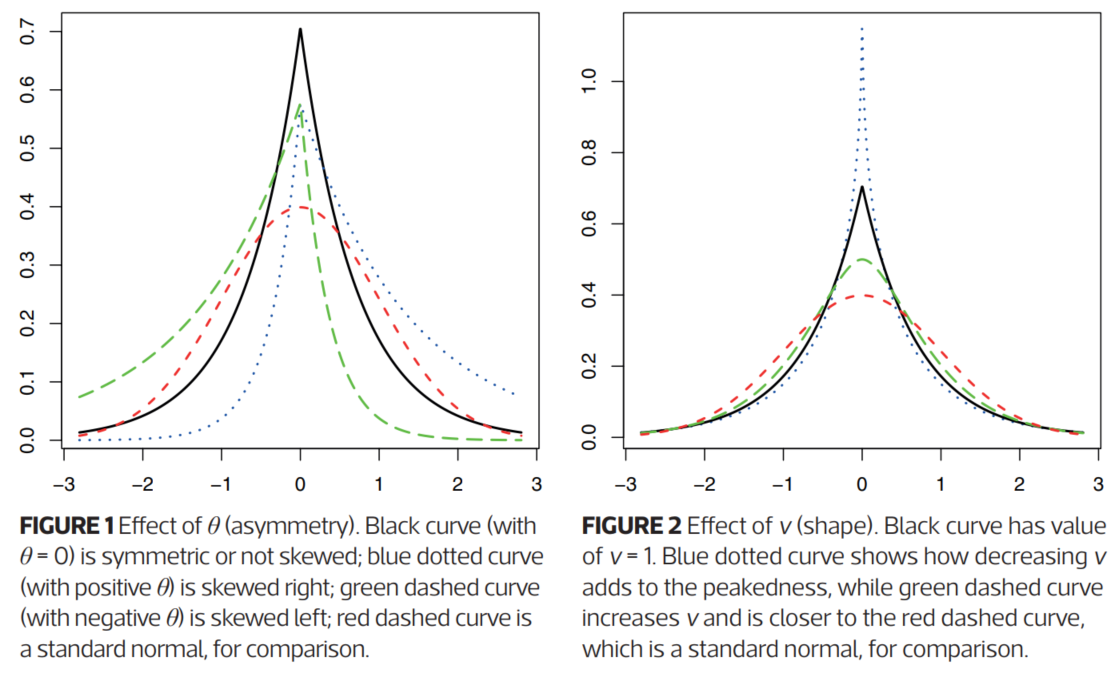
\includegraphics[width=0.7\linewidth]{figure/vg_1} \end{center}
\end{frame}

\begin{frame}{Moments}
\protect\hypertarget{moments}{}
Cannot be completely described by the first two moments, mean and
variance The shape parameter \(\nu\) for kurtosis to the normal
distribution with a kurtosis of 3 With an assumed small skewness
(\(\theta\))

The first four moments of the VG are:

\begin{enumerate}
\tightlist
\item
  mean: \(E[X_t] = \mu + \theta\)
\item
  variance: \(Var[X_t] = \sigma^2\)
\item
  skewness: \(\gamma[X_t] = 3\theta\nu/\sigma\)
\item
  kurtosis: \(\kappa[X_t] = 3(1 + \nu)\)
\end{enumerate}
\end{frame}

\begin{frame}{Summary}
\protect\hypertarget{summary}{}
Three common ways to simulate from the VG distribution are:

\begin{enumerate}
\item
  As a time-changed Brownian motion with a gamma
\item
  The difference of two non-decreasing (Gamma) processes
\item
  Using a compound Poisson process, for an approximation
\end{enumerate}

An R package, VarianceGamma (bit.ly/2NZZnJ2), includes the ability to
estimate parameters from data and also simulate random variates.
\end{frame}

\hypertarget{bessel-function}{%
\section{Bessel function}\label{bessel-function}}

\begin{frame}{}
\protect\hypertarget{section-1}{}
\begin{center}\includegraphics[width=0.7\linewidth]{11_gamma_bessel_files/figure-beamer/unnamed-chunk-2-1} \end{center}
\end{frame}

\begin{frame}{}
\protect\hypertarget{section-2}{}
\begin{center}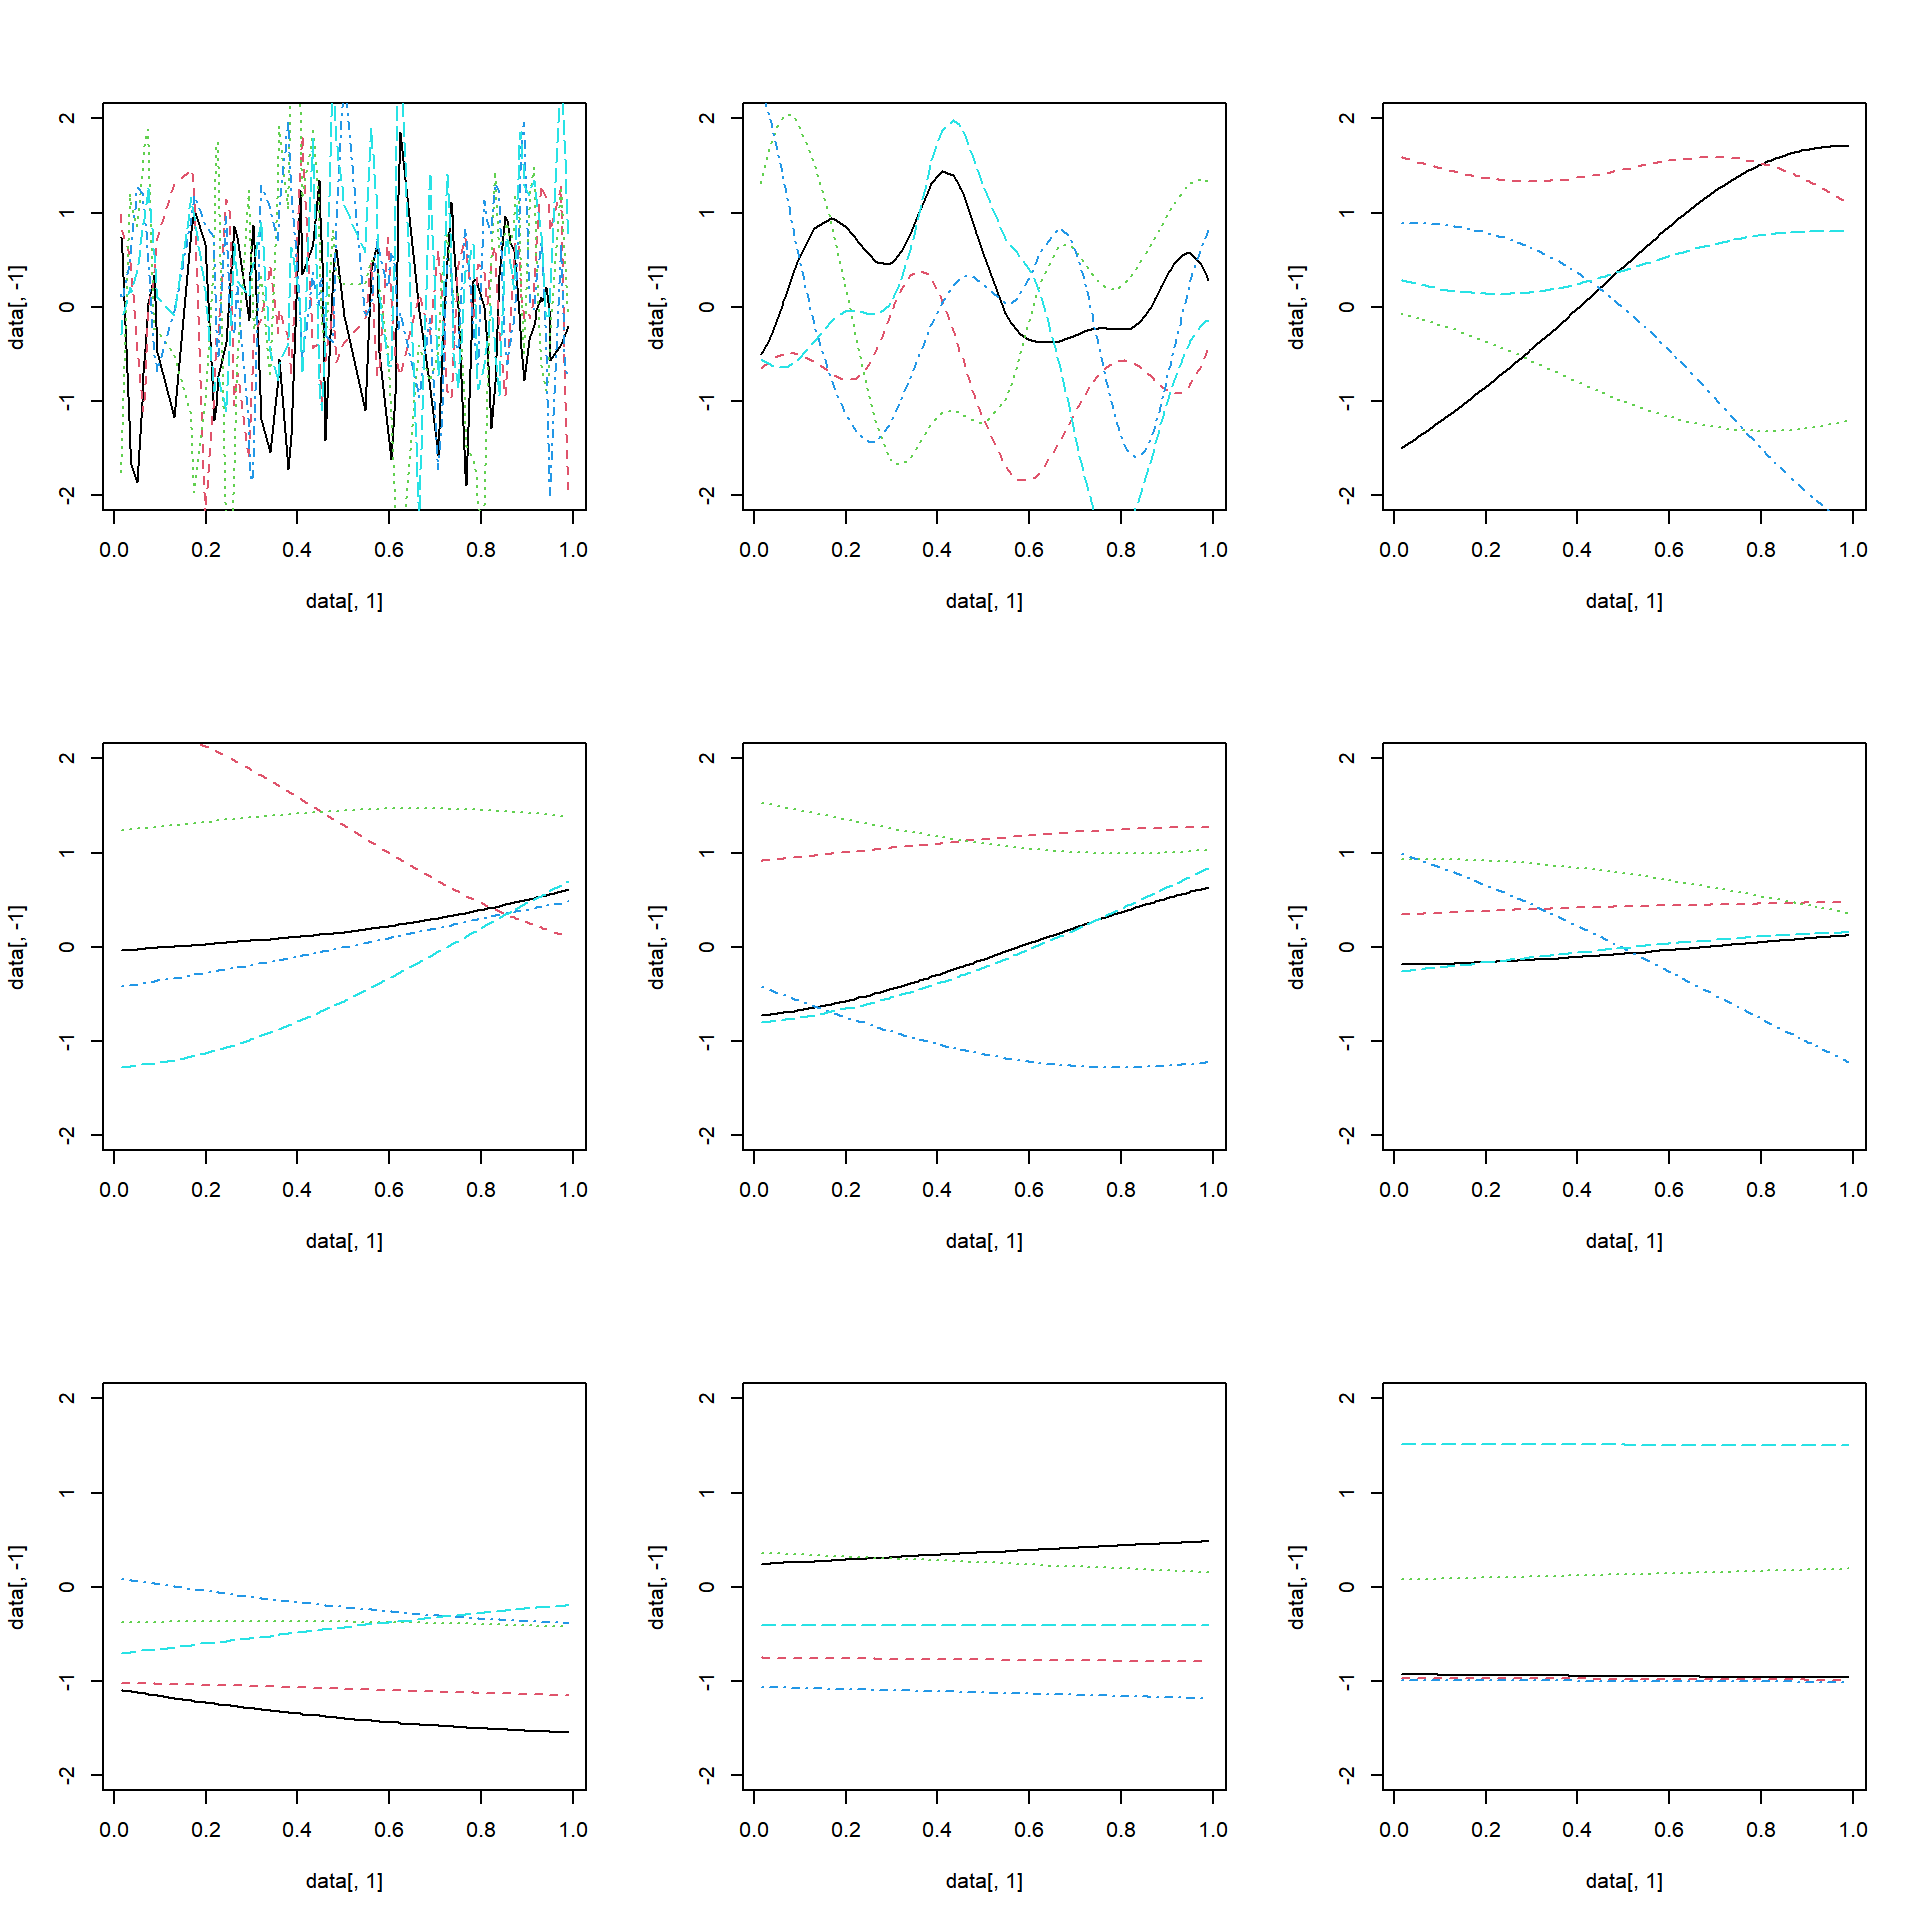
\includegraphics[width=0.7\linewidth]{11_gamma_bessel_files/figure-beamer/unnamed-chunk-3-1} \end{center}
\end{frame}

\begin{frame}{}
\protect\hypertarget{section-3}{}
\begin{center}\includegraphics[width=0.7\linewidth]{11_gamma_bessel_files/figure-beamer/unnamed-chunk-4-1} \end{center}
\end{frame}

\begin{frame}{}
\protect\hypertarget{section-4}{}
\begin{center}\includegraphics[width=0.7\linewidth]{11_gamma_bessel_files/figure-beamer/unnamed-chunk-5-1} \end{center}
\end{frame}

\begin{frame}{}
\protect\hypertarget{section-5}{}
\begin{center}\includegraphics[width=0.7\linewidth]{11_gamma_bessel_files/figure-beamer/unnamed-chunk-6-1} \end{center}
\end{frame}

\begin{frame}{}
\protect\hypertarget{section-6}{}
\begin{center}\includegraphics[width=0.7\linewidth]{11_gamma_bessel_files/figure-beamer/unnamed-chunk-7-1} \end{center}
\end{frame}

\begin{frame}{}
\protect\hypertarget{section-7}{}
\begin{center}\includegraphics[width=0.7\linewidth]{11_gamma_bessel_files/figure-beamer/unnamed-chunk-8-1} \end{center}
\end{frame}

\begin{frame}{}
\protect\hypertarget{section-8}{}
\begin{center}\includegraphics[width=0.7\linewidth]{11_gamma_bessel_files/figure-beamer/unnamed-chunk-9-1} \end{center}
\end{frame}

\end{document}
